% ==========================================
% BAB II STUDI LITERATUR
% ==========================================
\chapter{STUDI LITERATUR}
\label{chap:studi-literatur}

\section{\textit{Spyware}}
\subsection{Definisi dan Karakteristik \textit{Spyware}}

Menurut \textcite{reddy2024review}, \textit{spyware} secara umum 
didefinisikan sebagai salah satu bentuk \textit{malicious software} 
(\textit{malware}) yang dirancang untuk memantau, merekam, dan 
mengirimkan informasi sensitif pengguna tanpa sepengetahuan maupun 
persetujuan pemilik perangkat. Kondisi ini menimbulkan ancaman serius 
terhadap kerahasiaan data dan privasi digital. Dalam ranah 
\textit{cyber espionage}, \textit{spyware} modern telah berevolusi 
menjadi alat intelijen siber berkapabilitas tinggi. Pegasus, 
misalnya, merupakan \textit{advanced spyware} yang mampu menginfeksi 
\textit{smartphone} melalui berbagai vektor serangan dan mengekstraksi 
hampir seluruh jenis data, termasuk komunikasi terenkripsi, sehingga 
ancamannya mencakup individu, organisasi, hingga level negara 
\autocite{kareem2024pegasus}. Dengan kemampuan pengawasan jangka 
panjang, pelacakan lokasi, serta pemantauan aktivitas secara 
\textit{real time}, \textit{spyware} menempati posisi penting 
dalam ekosistem ancaman keamanan modern.

Secara karakteristik, \textit{spyware} biasanya memiliki kemampuan 
untuk beroperasi secara tersembunyi (\textit{stealth}), bertahan 
lama (\textit{persistence}), serta melakukan komunikasi jarak jauh 
dengan server pengendali (\textit{command and control}) untuk mengirimkan 
data yang berhasil dikumpulkan \autocite{salih2020spyware}. Pada platform 
Android, \textit{spyware} kerap disisipkan ke dalam aplikasi palsu atau 
aplikasi yang tampak fungsional, lalu meminta berbagai \textit{permission} 
sensitif, seperti akses kontak, pesan, lokasi, kamera, dan mikrofon 
sebagai bagian dari \textit{social engineering}.

\textcite{kareem2024pegasus} menambahkan bahwa \textit{spyware} tingkat lanjut dapat 
memanfaatkan kerentanan \textit{zero day} dan mekanisme serangan 
\textit{zero click} sehingga mampu menginfeksi perangkat tanpa perlu 
interaksi pengguna, sekaligus menghapus jejak untuk mengurangi kemungkinan 
analisis forensik. Dari sisi perilaku, \textit{spyware} umumnya menargetkan 
berbagai jenis data, mulai dari kredensial, pesan instan, email, daftar 
kontak, log panggilan, riwayat penelusuran, hingga data sensor seperti 
lokasi GPS dan rekaman audio atau video. Beberapa implementasi juga 
menyertakan fungsi \textit{keylogging}, pengambilan \textit{screenshot}, 
dan pengumpulan informasi perangkat yang kemudian dimanfaatkan untuk 
\textit{profiling} target serta perencanaan serangan lanjutan.

\subsection{\textit{Spyware} Mode \textit{Stealth}}

\textcite{elghaly2024fileless} menjelaskan bahwa \textit{spyware} mode 
\textit{stealth} merujuk pada kelas \textit{spyware} yang dirancang untuk 
beroperasi secara terselubung dengan meminimalkan jejak artefak forensik, sehingga 
sulit terdeteksi oleh pengguna maupun solusi keamanan seperti antivirus 
dan \textit{Endpoint Detection and Response} (EDR). Salah satu ciri 
utama mode \textit{stealth} adalah pemanfaatan teknik \textit{fileless} 
dan \textit{living off the land}, yaitu menjalankan \textit{payload} 
langsung di memori serta menyalahgunakan komponen bawaan sistem seperti 
PowerShell, WMI, dan \textit{task scheduler}, sehingga tidak meninggalkan 
berkas \textit{executable} mencolok di disk. Dari sisi teknik, 
\autocite{elghaly2024fileless} mendeskripsikan bahwa mode \textit{stealth} sering 
bergantung pada beberapa mekanisme: eksekusi \textit{in memory}, 
\textit{code obfuscation}, penggunaan komunikasi terenkripsi, serta 
pemanfaatan \textit{persistence} yang terselubung melalui \textit{registry}, 
\textit{scheduled task}, atau \textit{startup folder} yang tidak secara 
eksplisit menunjukkan nama \textit{malware}.

\textit{Spyware} canggih seperti Pegasus menggabungkan kemampuan penyamaran 
proses, enkripsi komunikasi, dan mekanisme \textit{self-destruct} untuk 
mempertahankan \textit{persistence} sekaligus menghapus bukti ketika 
upaya analisis terdeteksi \autocite{kareem2024pegasus}. Pada kasus Pegasus, 
aspek \textit{stealth} mencakup penggunaan \textit{exploit zero click}, 
penyamaran sebagai proses sistem yang sah, komunikasi \textit{command and 
control} (C2) terenkripsi, serta kemampuan untuk menyesuaikan diri dengan 
lingkungan target dan menghilang ketika indikator analisis terdeteksi. 
\textit{Spyware} ini juga memanfaatkan berbagai vektor infeksi seperti 
\textit{phishing}, \textit{exploit chain}, \textit{watering hole attacks}, 
dan \textit{network injection} sehingga proses infeksi dapat terjadi tanpa 
interaksi pengguna, memperkuat karakteristik \textit{stealth} baik pada 
fase infeksi maupun fase operasi pengumpulan data.

\Textcite{sudhakar2020fileless} menjelaskan bahwa \textit{fileless malware} 
dirancang untuk beroperasi langsung di memori dengan memanfaatkan komponen 
bawaan sistem seperti PowerShell dan Windows Management Instrumentation 
(WMI), sehingga hampir tidak meninggalkan berkas tradisional di disk. 
Karakteristik ini menjadikan \textit{fileless malware} sulit dideteksi 
oleh solusi keamanan berbasis \textit{signature} dan selaras dengan tujuan 
operasi \textit{stealth} karena aktivitas berbahaya berbaur dengan aktivitas 
administratif yang sah.

\section{\textit{Data Crawling}}
\subsection{Definisi \textit{Data Crawling}}

Data \textit{crawling} adalah proses otomatis yang dilakukan untuk 
mengumpulkan data dari berbagai sumber, terutama dari internet atau sistem 
digital, dengan cara menjelajahi dan mengambil konten secara sistematis 
menggunakan perangkat lunak khusus yang disebut \textit{crawler}. Proses 
ini memungkinkan pengumpulan informasi yang kemudian dapat dianalisis lebih 
lanjut untuk berbagai keperluan, termasuk dalam ranah keamanan siber dan 
intelijen digital \autocite{salih2020spyware}. Dalam konteks siber, 
\textit{crawling} digunakan \textit{spyware} sebagai metode pengumpulan 
data korban secara tersembunyi dan berkelanjutan.

\textcite{kareem2024pegasus} menambahkan bahwa teknik \textit{crawling} pada 
\textit{spyware} modern seperti Pegasus diperluas dengan penggunaan metode 
eksfiltrasi data untuk memperluas jangkauan pengumpulan informasi, baik 
dari perangkat korban maupun sumber eksternal, sehingga efektivitas 
pengintaian digital semakin meningkat.

Menurut \textcite{jegan2024aicrawler}, \textit{crawling} dipahami sebagai proses 
penelusuran data yang dilakukan secara otomatis, terstruktur, dan berulang 
untuk menjangkau berbagai informasi digital. Sistem \textit{crawling} 
dirancang untuk menavigasi dan menelusuri struktur data, baik dalam bentuk 
jaringan, tautan, maupun elemen-elemen sistem lain, untuk mengekstraksi 
konten serta mengidentifikasi pola atau informasi penting dari sumber data 
yang kompleks. Konsep ini sejalan dengan pemanfaatan \textit{crawling} 
dalam perangkat lunak berbahaya, di mana prinsip \textit{systematic 
traversal} yang digunakan pada \textit{web crawling} juga diterapkan pada 
lingkungan perangkat korban, misalnya dengan menelusuri direktori, memindai 
berkas, membaca metadata, atau mengakses \textit{cache} aplikasi.

\subsection{Jenis Data Target \textit{Crawling}}
Menurut penelitian yang dilakukan \textcite{salih2020spyware}, 
\textit{spyware} Android yang mereka kembangkan dan uji disembunyikan 
di dalam aplikasi permainan palsu dengan tujuan memperoleh berbagai 
informasi korban, seperti kontak, pesan, panggilan, akun, serta lokasi 
geografis melalui Wi-Fi atau SIM, 3G, 4G, dan LTE, serta informasi pribadi 
lain yang tersimpan di perangkat. Selain itu, \textit{spyware} tersebut 
juga dapat menampilkan daftar korban, mengambil seluruh kontak, membaca 
pesan masuk dan keluar, serta melihat \textit{call log}.

\textcite{kareem2024pegasus} menjelaskan bahwa Pegasus, setelah berhasil menginfeksi 
\textit{smartphone}, mampu mengakses berbagai jenis data sensitif dari 
perangkat target, termasuk pesan, email, panggilan, riwayat penelusuran, 
data dari aplikasi media sosial, serta data dari aplikasi pesan terenkripsi. 
\textcite{kareem2024pegasus} juga menyebutkan bahwa Pegasus dapat mengaktifkan mikrofon 
dan kamera untuk merekam audio dan video, melacak lokasi secara 
\textit{real time}, menangkap penekanan tombol, serta mengumpulkan berkas 
dan pengenal unik perangkat.

\subsection{Teknik dan Mekanisme \textit{Data Crawling}}

Teknik dan mekanisme \textit{data crawling} dalam konteks \textit{spyware} 
dan keamanan siber menggambarkan bagaimana sistem berbahaya maupun 
\textit{security monitoring tools} mengotomatisasi proses pengumpulan 
informasi dari perangkat korban. Menurut \textcite{salih2020spyware}, teknik 
\textit{crawling} pada \textit{spyware} Android diimplementasikan dengan 
menyisipkan kode \textit{spyware} ke dalam aplikasi permainan palsu yang 
berjalan seperti aplikasi biasa namun di latar belakang mengeksekusi fungsi 
pengambilan data. Saat aplikasi dibuka, \textit{spyware} secara otomatis 
mengumpulkan kontak, pesan, \textit{call log}, akun, dan lokasi, kemudian 
mengirimkannya ke \textit{REST API} berbasis PHP yang menyimpan data 
tersebut pada basis data MySQL sehingga operator dapat mengaksesnya melalui 
\textit{control panel} tanpa memerlukan interaksi tambahan dengan korban.

Pada \textit{spyware} Pegasus, setelah tahap infeksi, \textit{spyware} 
menjalankan modul untuk mengekstraksi berbagai jenis data dari perangkat 
target. Pada bagian \textit{data collection and exfiltration}, 
\textcite{kareem2024pegasus} menjelaskan bahwa Pegasus mengakses pesan instan, media 
sosial, riwayat penelusuran, sandi tersimpan, kalender, catatan, pengenal 
perangkat, serta berkas lokal maupun \textit{cloud}. Data tersebut kemudian 
dienkripsi dan dikirimkan ke server \textit{command and control} (C2) 
sebagai mekanisme eksfiltrasi yang terotomatisasi dan berulang.

Penelitian yang dilakukan \textcite{jegan2024aicrawler} secara spesifik membahas 
mekanisme \textit{web crawling} pada lingkungan \textit{dark web}, yaitu 
proses penelusuran otomatis terhadap halaman dan tautan untuk mengumpulkan 
informasi seperti kredensial yang terekspos dan diskusi terkait serangan 
siber. Mekanisme \textit{data crawling} dalam sistem mereka dimulai dari 
pemberian kata kunci atau URL awal yang kemudian digunakan \textit{crawler} 
untuk menelusuri \textit{dark web} dan mengekstraksi informasi penting 
seperti \textit{compromised credentials}. \textit{Crawler} secara otomatis 
mengirim \textit{HTTP request}, mengambil halaman, mengekstrak konten, 
kemudian memanfaatkan \textit{natural language processing} (NLP) dan 
\textit{machine learning} (ML) untuk menginterpretasi data tidak 
terstruktur serta mendeteksi pola anomali yang mengindikasikan potensi 
ancaman.

\section{\textit{Exfiltration}}
\subsection{Definisi dan Tujuan \textit{Exfiltration}}

\begin{figure}[H]
    \centering
    \captionsetup{justification=centering}
    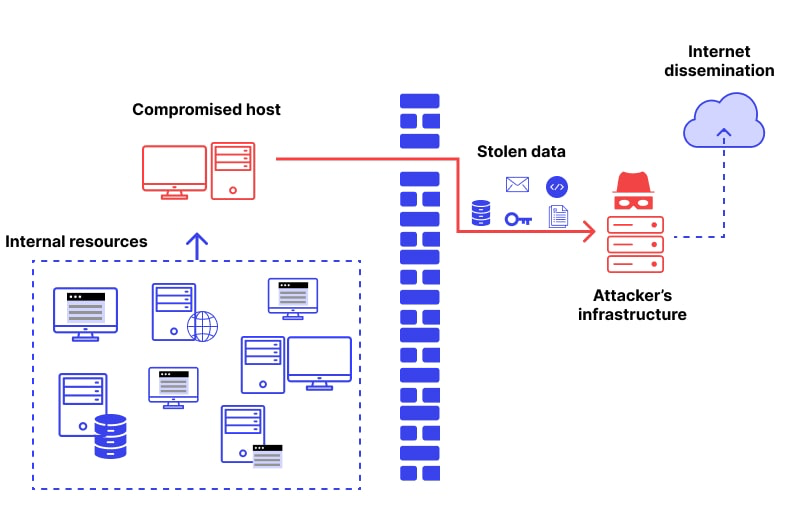
\includegraphics[width=0.85\textwidth]{image/exfiltration.png}
    \caption{Data \textit{Exfiltration}}
    \label{fig:exfiltration}
\end{figure}

Definisi dan tujuan eksfiltrasi dalam konteks \textit{spyware} dan 
keamanan siber merujuk pada proses pengambilan dan pengiriman keluar 
data dari sistem atau perangkat target secara tidak sah oleh pihak 
penyerang. \textcite{reddy2024review} menjelaskan eksfiltrasi sebagai salah satu 
aktivitas utama \textit{payload} \textit{spyware}, yaitu pengambilan dan 
pengiriman keluar data sensitif secara tidak sah setelah \textit{spyware} 
berhasil dijalankan di dalam sistem korban. \textit{Spyware} pada perangkat 
yang telah terkompromi mengakses berbagai sumber daya internal, mengumpulkan 
data sensitif, kemudian mengirimkannya keluar melewati batas jaringan 
menuju infrastruktur penyerang. Data yang telah dieksfiltrasi tersebut 
selanjutnya dapat dimanfaatkan sesuai tujuan penyerang.

Menurut \textcite{king2021dataexfiltration}, \textit{data exfiltration} didefinisikan 
sebagai proses pemindahan data secara tidak sah dari dalam jaringan atau 
sistem organisasi ke pihak luar melalui berbagai media dan protokol 
komunikasi. Eksfiltrasi merupakan tahap akhir dari banyak insiden keamanan, 
ketika pelaku yang telah memperoleh akses berusaha mengeluarkan informasi 
bernilai tinggi. Tujuan utama \textit{exfiltration} adalah mengumpulkan 
dan mengirimkan data bernilai ke infrastruktur penyerang untuk kemudian 
dimonetisasi, dimanfaatkan dalam spionase, atau digunakan sebagai 
\textit{leverage} dalam pemerasan. Proses eksfiltrasi dijaga kerahasiaannya 
dengan menyamarkan lalu lintas keluar agar terlihat seperti trafik normal, 
misalnya dengan memanfaatkan protokol umum serta pola komunikasi yang 
menyerupai aktivitas sah di jaringan.

\subsection{Metode \textit{Exfiltration}}

\textcite{king2021dataexfiltration} menjelaskan bahwa metode \textit{data exfiltration} 
dapat dikategorikan menjadi tiga kelompok utama, yaitu 
\textit{content-based}, \textit{header-based}, dan \textit{meta-based 
methods}. Dalam studi tersebut, diimplementasikan beberapa teknik 
eksfiltrasi, seperti penyisipan data pada citra digital (\textit{image 
steganography}), pemanfaatan HTTP~404 untuk menyamarkan transfer data 
pada \textit{web logs}, manipulasi nilai \textit{Time To Live} (TTL), 
manipulasi \textit{IP options field}, serta pemanfaatan \textit{e-mail 
header} untuk membawa \textit{payload} eksfiltrasi sebelum kemudian diuji 
apakah serangan tersebut dapat dideteksi oleh IDS Snort.

\textcite{ullah2018dataexfiltration} mengulas berbagai vektor serangan eksternal yang 
digunakan untuk eksfiltrasi data, antara lain \textit{web-based 
exfiltration} melalui HTTP/HTTPS, eksfiltrasi berbasis \textit{e-mail}, 
\textit{DNS tunneling}, protokol \textit{file transfer}, layanan 
\textit{cloud storage} dan \textit{file sharing}, serta berbagai 
\textit{covert channels}. Penulis menekankan bahwa penggunaan protokol 
dan layanan yang umum digunakan organisasi, seperti HTTP/HTTPS dan layanan 
\textit{cloud}, membuat lalu lintas eksfiltrasi sulit dibedakan dari trafik 
sah, sehingga setiap vektor dibahas bersamaan dengan ringkasan 
\textit{countermeasures} yang dapat diterapkan.

Penelitian oleh \textcite{zhan2022doh} menunjukkan bahwa penyerang dapat 
memanfaatkan \textit{DNS over HTTPS} (DoH) sebagai kanal eksfiltrasi 
dengan menyembunyikan permintaan DNS di dalam trafik HTTPS terenkripsi. 
Studi ini menganalisis karakteristik trafik DoH, meliputi \textit{TLS 
fingerprint} dan fitur-fitur aliran (\textit{flow-based features}) yang 
berbeda dari pola penggunaan normal, serta mengusulkan metode deteksi 
berbasis \textit{machine learning} untuk mengidentifikasi \textit{DoH 
tunneling}.

\section{\textit{Anti-Spyware}}
\subsection{Definisi \textit{Anti-Spyware}}

\textcite{baldota2025review} menyatakan bahwa \textit{anti-spyware} merupakan 
perangkat lunak atau mekanisme keamanan yang dirancang khusus untuk 
mengidentifikasi, menghapus, dan mencegah aktivitas \textit{spyware} 
dalam sistem komputer maupun perangkat bergerak. Fungsi utama 
\textit{anti-spyware} tidak hanya mendeteksi dan menghapus program 
\textit{spyware} yang berbahaya, tetapi juga melindungi privasi pengguna 
serta mencegah pencurian data secara diam-diam oleh aplikasi tidak sah. 
Perangkat \textit{anti-spyware} dilengkapi dengan berbagai teknik, mulai 
dari \textit{signature-based detection}, \textit{behavior-based detection}, 
\textit{heuristics}, hingga metode berbasis \textit{machine learning} 
untuk memperluas jangkauan dan efektivitas deteksi terhadap beragam varian 
\textit{spyware} yang terus berkembang. Selain peran deteksi dan penghapusan, 
\textit{anti-spyware} juga berfungsi memperkuat lapisan keamanan digital 
dengan mencegah eksekusi maupun inisiasi aktivitas \textit{spyware} lebih 
lanjut di perangkat korban. Dengan integrasi ke pengamanan \textit{endpoint} 
dan pengawasan aplikasi, \textit{anti-spyware} menjadi bagian penting dari 
strategi proteksi data modern.

\textcite{qabalin2022android} menekankan bahwa modul deteksi \textit{spyware} 
merupakan inti dari mekanisme \textit{anti-spyware} dalam ekosistem 
perangkat Android. Dengan kemampuan membedakan aplikasi \textit{spyware} 
dari aplikasi resmi, \textit{anti-spyware} menjaga perlindungan perangkat 
agar terbebas dari ancaman pengumpulan data tersembunyi oleh program jahat. 
Sistem \textit{anti-spyware} dirancang untuk mengenali ciri-ciri aplikasi 
yang melakukan pemantauan, pengumpulan informasi, perekaman aktivitas, atau 
perubahan pengaturan tanpa persetujuan pengguna sebagai bagian dari fungsi 
pengintaian.

\subsection{Mekanisme Deteksi \textit{Anti-Spyware}}
Untuk mengidentifikasi dan mencegah aktivitas pengintaian yang dilakukan 
\textit{spyware}, berbagai mekanisme deteksi telah dikembangkan dalam 
solusi keamanan modern. Setiap mekanisme berupaya mengenali keberadaan 
\textit{spyware} melalui pendekatan yang berbeda, baik dengan mencocokkan 
ciri khas \textit{malware} yang sudah diketahui, menganalisis perilaku 
mencurigakan selama program berjalan, maupun menilai karakteristik yang 
tidak biasa berdasarkan aturan dan skor tertentu. Beberapa penelitian juga 
mengusulkan pemanfaatan teknik pembelajaran mesin untuk meningkatkan akurasi 
deteksi terhadap varian \textit{spyware} baru yang sulit dikenali dengan 
metode tradisional. Secara umum, mekanisme deteksi \textit{anti-spyware} 
dapat dikelompokkan ke dalam \textit{signature-based detection}, 
\textit{behavior-based} dan \textit{heuristic detection}, pendekatan 
\textit{machine learning-based detection}, serta deteksi berbasis trafik jaringan.

\begin{enumerate}
    \item \textit{Signature Based Detection}

    Menurut \textcite{baldota2025review}, banyak solusi \textit{anti-spyware} tradisional 
    mengandalkan \textit{signature-based detection}, yaitu mencocokkan pola 
    biner atau ciri khas \textit{spyware} yang sudah diketahui dengan berkas 
    atau proses yang sedang diperiksa. Pendekatan ini efektif untuk 
    \textit{spyware} yang sudah dikenal, tetapi kurang mampu mendeteksi 
    varian baru atau \textit{spyware} yang di-\textit{obfuscate} karena 
    tidak memiliki \textit{signature} yang tersimpan di basis data.

    \item \textit{Behavior Based dan Heuristic Detection}

    \textit{Behavior-based detection} memonitor aktivitas program, seperti 
    akses berkas, perubahan \textit{registry}, koneksi jaringan, dan 
    interaksi dengan API sistem, untuk mengidentifikasi pola perilaku 
    yang menyerupai \textit{spyware}, misalnya pengambilan data sensitif 
    atau aktivitas tersembunyi. Mekanisme ini sering dipadukan dengan 
    \textit{heuristic detection}, yang menggunakan aturan atau 
    \textit{scoring} untuk menilai apakah kombinasi perilaku tertentu 
    cukup mencurigakan untuk dikategorikan sebagai ancaman \autocite{baldota2025review}.

    \item \textit{Machine Learning Based Detection}

    Pendekatan modern banyak memanfaatkan algoritma \textit{machine 
    learning} untuk membedakan \textit{spyware} dari aplikasi resmi 
    berdasarkan fitur statis maupun dinamis \autocite{baldota2025review}. 
    Penelitian yang dilakukan oleh \textcite{abualhaj2024decisiontree} menunjukkan 
    bahwa model \textit{decision tree} yang dioptimalkan mampu 
    mengklasifikasikan sampel \textit{spyware} dengan akurasi tinggi 
    pada dataset \textit{malware}, sehingga dapat dijadikan modul deteksi 
    pada sistem \textit{anti-spyware}. Sementara itu, penelitian oleh 
    \textcite{wang2025atsdetector} mengembangkan deteksi \textit{Trojan spyware} 
    Android dengan menggabungkan fitur statis seperti \textit{permission} 
    dan metadata aplikasi serta fitur dinamis dari perilaku 
    \textit{runtime}, kemudian melatih model \textit{machine learning} 
    untuk membedakan \textit{spyware} dari aplikasi \textit{benign}.

    \item Deteksi Berbasis Trafik Jaringan

    Metode SNDMI yang diperkenalkan dalam penelitian oleh \textcite{peng2024sndmi} 
    memfokuskan deteksi \textit{spyware} pada analisis pola trafik jaringan, 
    termasuk penggunaan trafik \textit{inducement} dan fitur-fitur 
    \textit{flow} untuk melatih model LightGBM. Pendekatan ini menempatkan 
    modul deteksi di level jaringan sehingga \textit{spyware} dapat 
    diidentifikasi melalui pola komunikasi ke server eksternal tanpa harus 
    selalu bergantung pada inspeksi berkas atau proses pada \textit{endpoint}.

\end{enumerate}

\section{Studi Sebelumnya}

Studi sebelumnya diperlukan untuk memahami perkembangan penelitian 
terkait \textit{data crawling}, mekanisme pengumpulan data oleh 
\textit{spyware}, serta berbagai teknik eksfiltrasi dan deteksi yang 
digunakan dalam keamanan siber. Kajian ini memberikan gambaran mengenai 
pendekatan, metode, serta keterbatasan penelitian terdahulu yang menjadi 
dasar dalam merumuskan ruang lingkup dan kontribusi penelitian ini.

\captionsetup{justification=raggedright,singlelinecheck=false}
\begin{longtable}{|p{0.5cm}|p{3cm}|p{2.3cm}|p{3.6cm}|p{3.6cm}|}
\caption{Studi Sebelumnya}
\label{tbl:studi-sebelumnya} \\
\hline
\textbf{No} &
\textbf{Judul Penelitian (Penulis)} &
\textbf{Metode} &
\textbf{Hasil Utama} &
\textbf{Keterbatasan} \\
\hline
\endfirsthead

\hline
\textbf{No} &
\textbf{Judul Penelitian (Penulis)} &
\textbf{Metode} &
\textbf{Hasil Utama} &
\textbf{Keterbatasan} \\
\hline
\endhead

\hline
\endfoot

1 &
\textit{Design and Implementation of an Android Spyware Application Using a Fake Game} \autocite{salih2020spyware} &
Perancangan sistem dan eksperimen &
Mengembangkan \textit{spyware} Android yang melakukan \textit{data crawling} terhadap kontak, pesan, \textit{log} panggilan, akun, dan lokasi, serta mengekstraksinya secara otomatis ke server \textit{backend} melalui REST API &
Berfokus pada Android saja, tidak membahas mekanisme \textit{stealth} tingkat lanjut atau deteksi oleh \textit{anti-spyware}. \\
\hline

2 &
\textit{Cyber Threat Intelligence through Automated Dark Web Crawling} \autocite{jegan2024aicrawler} &
Perancangan sistem dan eksperimen &
Mengimplementasikan \textit{web crawling} otomatis pada \textit{dark web} dengan ekstraksi konten, pemetaan tautan, dan deteksi kredensial yang terekspos menggunakan \textit{machine learning}. &
Fokus pada \textit{crawling} di \textit{dark web} untuk CTI, bukan \textit{crawling} internal pada perangkat korban seperti \textit{spyware}. \\
\hline

3 &
\textit{Stealthy Data Collection and Exfiltration in Pegasus Spyware} \autocite{kareem2024pegasus} &
Studi literatur teknis dan analisis arsitektur &
Mendeskripsikan mekanisme \textit{data collection} dan \textit{auto-exfiltration} \textit{spyware} Pegasus, mencakup akses pesan, email, media sosial, \textit{keylogging}, rekaman audio/video, lokasi \textit{real-time}, serta pengiriman terenkripsi ke C2. &
Tidak menyertakan implementasi uji empiris; sebagian informasi berasal dari laporan investigatif, bukan eksperimen langsung. \\
\hline

4 &
\textit{An Emerging Threat: Fileless Malware -- A Survey and Research Challenges} \autocite{sudhakar2020fileless} &
Studi literatur &
Menjelaskan teknik penyembunyian dan eksfiltrasi \textit{fileless}, termasuk penggunaan \textit{PowerShell}, \textit{registry abuse}, dan \textit{memory-resident payload}. &
Tidak membahas implementasi \textit{crawling} secara spesifik atau eksfiltrasi berbasis protokol tertentu. \\
\hline

\end{longtable}